The goal of this chapter is to give a detailed description of the \textit{Bacco} protocol and to discuss the
implementation choices that were taken in order to deploy it. This is achieved using a top-down ordering for the level
of detail, meaning that an overview of the network is to be presented before going into the specifics.

\section{Overview}
The network is built upon 3 fundamental categories of devices:

\begin{description}[font=$\bullet$~\normalfont\scshape\color{blue!50!black}]
    \item [Sender node] - collects data and sends it to the gateway using LoRa
    \item [Repeater node] - listens to the incoming LoRa messages and repeates them
    \item [Gateway node] - collects data coming from the sender nodes and sends it to the web server using the FTP
        protocol over a mobile network such as \gls{GSM} or \gls{LTE} \footnote{A gateway can be configured to optionally perform
        some operation or elaboration (e.g.: filtering, smoothing, pre-processing, ...) of the incoming data and can
    even collect relevant data on-site.}
    \item [Web server] - receives data coming from the gateways through FTP, elaborates it and makes it available to
        consult through a self-hosted web application platform
\end{description}

\begin{figure}[ht]
    \centering
    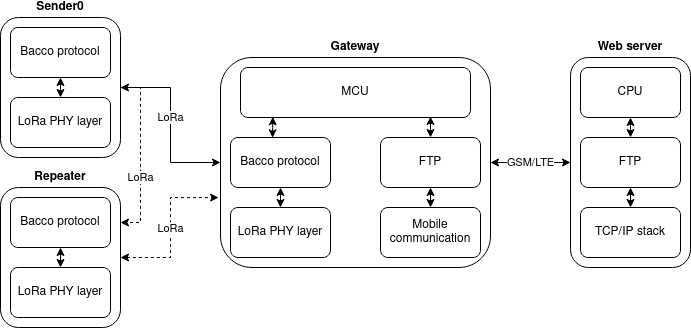
\includegraphics[width=1.0\textwidth]{uml/network_stack.png}
    \caption{Schematic representation of the used protocols}
    \label{network stack img}
\end{figure}

\subsection{Topology}
The network has a 2 layered star-of-stars topology, and can make use of LoRa repeaters where physical obstacles or range
compromise the integrity of the communication channel (e.g.: hills, thick brick walls, ...). Figure \ref{network
topology img} shows the type of devices that are involved and their communication schema.

\begin{figure}[ht]
    \centering
    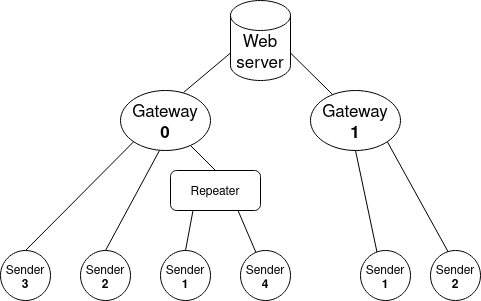
\includegraphics[width=200pt]{uml/network_topology.png}
    \caption{Network topology}
    \label{network topology img}
\end{figure}

%TODO: remove, jsut for test
\subsection{TODO: REMOVE}
\gls{latex}
